\chapter{Problem Definition}
\label{chapter3}
\thispagestyle{empty}

\begin{quotation}
{\footnotesize
\noindent{\emph{``\greek{p'antec >'anjrwpoi to~u e>id'enai >or'egontai f'usei}''}\\
(All men naturally desire knowledge)}
\begin{flushright}
\greek{>Aristot'elhc}(Aristotle, Met. 1.980a)
\end{flushright}
}
\end{quotation}


%\noindent In questa sezione si deve descrivere l'obiettivo della ricerca, le problematiche affrontate ed eventuali definizioni preliminari nel caso la tesi sia di carattere teorico.
The aim of our work is to analyze the performances of mitosis detection algorithms compared to humans trying to classify the same images.
To acheve this goal, we selected a subset of the publicly-available \textit{MITOS dataset} made for the \textit{ICPR 2012 Contest} on
\texttt{Mitosis Detection in Breast Cancer Histological Images}\footnote{\url{http://ipal.cnrs.fr/ICPR2012/}}.
Then we run the following activities:

\begin{itemize}
 \item collected the performances of the top-scoring algorithms developed for the ICPR 2012 Mitosis Detection Contest (focusing on the dataset),
 \item applied some classifiers to the dataset,
 \item implemented a web-based test for humans,
 \item analyzed the performances of the algorithms compared to the results achieved by humans.
\end{itemize}

The main definitions for the problem in exam are the subject of this chapter.

\section{Framework}


The purpose of automating the mitosis detection problem requires the definition of a framework that involves Computer Vision and Machine Learning aspects.
\Gls{ML} is growing in importance for biology-related tasks \cite{tarca2007machine}.
In general, \Gls{PR} (see \ref{ch2:pr}) is the computational approach used to analyze datasets of images \cite{patternRecSWBioImages01}.

\subsection{Detection}

The analysis of digital images requires identifying \Glspl{ROI} or \textit{candidates} within the images. Once a region is isolated,
a digital image allows many types of measurements and statistics to be collected, as well as the number of objects and their distribution.
This region selection can be done manually by drawing boxes or free-hand regions using an
interactive tool \cite{swedlow2009bioimage}, or automatically using
computer algorithms known as segmentation algorithms \cite{ljosa2009introduction}.
The input to the algorithm may be an entire image, a sub-image region identified with segmentation algorithms, or simply image samples
in the form of rectangular tiles.

\subsection{From Detection to Classification}

\Gls{PR} then requires training a computer to classify groups of images (i.e. a subset of images with manually detected mitoses).
The machine can learn on its own what aspects of the images represent natural experimental variation and are
therefore irrelevant, and what aspects are important for distinguishing the groups of
control images (i.e. the testing set) from each other (see \ref{ch3:class}).
This ability to select different image measurements  allows the use of a great
variety of image description algorithms, potentially making the collection of algorithms very general.
The benefits of subdividing images into \Glspl{ROI} involve:

\begin{itemize}
 \item reduce the number of pixels to consider
 \item bias the algorithm to process objects of interest rather than background
 \item center or align objects
\end{itemize}

A further step consists in the extraction of image content descriptors (\textit{image features}),
which are values that describe the image content numerically. These values can
reflect various texture parameters of the image, the statistical distribution of pixel intensities, edges, etc.
While the dimensionality of the raw pixels can be high, the number of image features ranges
between a dozen to a few hundred. Each feature value describes a specific image characteristic.
Then, the image features are used to draw conclusions about the data.
The feature set is then used to infer rules for combining them in a classifier.
These two steps constitute the training stage in PR, where the goal is to correctly
classify the training images. The trained classifier is then tested on control images
that were excluded from the training stage.
This cross-validation is important to establish the classifier's ability to identify
new images, ensuring that it is not restricted to recognizing images it was
trained with.

\subsection{Performances}

If the performance of the algorithm are not satisfying (see \ref{ch3:perf} for details), the algorithm can be trained again on a different set of features, until the
detection capabilities reach the desired values (if feasible).
Finally, the results of image classification
need to be interpreted by the researcher in
an experimental context to reach a biological conclusion. 
Figure \ref{ch3:fig1} shows the steps described above.

\clearpage


\begin{figure}[!hbt]
\centering

\begin{tikzpicture}[node distance = 2cm, auto]
    % Place nodes
    \node [cloud] (init) {Image data};
    \node [block, below of=init] (ROI) {ROI detection};
    \node [block, below of=ROI] (spl) {split data into training and test sets};
    \node [block, below of=spl] (ft) {Feature selection};
    \node [block, below of=ft] (train) {Training};
    \node [block, left of=train, node distance=4cm] (update) {model update};
    \node [block, below of=train] (test) {Testing};
    \node [decision, below of=test] (decide) {results OK?};
    \node [cloud, below of=decide, node distance=3.2cm] (stop) {biological inference};
    % Draw edges
    \path [line] (init) -- (ROI);
    \path [line] (ROI) -- (spl);
    \path [line] (spl) -- (ft);
    \path [line] (ft) -- (train);
    \path [line] (train) -- (test);
    \path [line] (test) -- (decide);
%     
    \path [line] (decide) -| node {no} (update);
    \path [line] (decide) -- node {yes}(stop);
    \path [line] (update) |- (ft);
    \path [line] (update) -- (train);

\end{tikzpicture}


\caption{Flowchart of Detection Algorithm}
\label{ch3:fig1}
\end{figure}


% \vspace{0.5cm}

\section{Definition of Classification}
\label{ch3:class}

In \Gls{ML} the idea of \textit{classification} refers to the problem of identifying to which of a set of categories
(named \textit{classe}s) a new observation belongs, on the basis of a training set of data containing instances whose category membership is known.
In case of mitosis detection, the elements of a classification are basically the following:

\begin{itemize}
\item the \textit{input} to the classification problem is a set of \textit{features} computed on each of the \textit{candidates} selected in a preparatory phase.
    Each set of features composing a candidate is known as \textit{instance}. Each instance is \textit{labeled}  with the \textit{class} which it belongs to.
\item the \textit{classes} are simply two: \texttt{mitosis} (which we call \textit{class 1} or \textit{positive})
    or \texttt{non-mitosis} (which we call \textit{class 0} or \textit{negative}) making it a case of binary classification.
\item the \textit{output} of the classification can be a \textit{hard} classification: the output of the classifier is simply \textit{0} or \textit{1},
    corresponding to mitosis or non-mitosis respectively. On the other hand the classification can be \textit{soft}: the output of the classifier is a real number \textit{c}:

\begin{equation}
 0 \leq c \leq 1
\end{equation}
a subsequent phase of analysis consists in selecting the best threshold so that:

\begin{equation}
   \textit{class}=\begin{cases}
    0, & \text{if $c<threshold$}.\\
    1, & \text{otherwise}.
  \end{cases}
\end{equation}
the selection of the threshold is made in function of the measured performances of the classification algorithm (see \ref{ch3:perf}).

\end{itemize}

\vspace{0.5cm}

\section{Review of Algorithms solving the mitosis detection problem}
\label{ch3:review}

Different to other pattern recognition tasks, mitotic cells essentially are irregular shape objects. As a result, there
is no simple or unique way of extracting the features of mitotic cells and then many different classifiers can be made.

Here we briefly review the main algorithms found in literature that solve the mitosis detection task.

\begin{itemize}
 \item[-] The method proposed in \cite{Mitosis01} consists of two main components: candidate extraction and candidate classification.
Candidate objects are extracted by image segmentation with the Chan-Vese level set method \cite{moelich2003tracking}.
A statistical classifier is trained with a number of features that describe the size, shape, color and texture of the candidate objects.
 \item[-] The approach in \cite{mitosisDetectBreastCancer01} uses, after a phase of automatic segmentation of the image, a \Gls{GGMM} to classify
the candidates: the \Gls{GGMM} is a parametric technique for estimating probability density function. In this context, it is formulated as a function of pixel intensities.
 \item[-] The work in \cite{breastCancerMitosisPCA_ICA} also proposes a two phases approach: the detection candidates points are selected by using
an algorithm named eXclusive Independent Component Analysis (XICA), which gives two sets of training patterns: positive and negative patterns (positive and negative basis set).
Then a sparse representation method \cite{wright2009robust} is used to classify the candidates.
 \item[-] Also the approach in \cite{irshad2011automated} has two phases.
In the first stage, the detection of candidate mitosis is performed. The input RGB
images are transformed into blue-ratio images. A Laplacian of Gaussian (LoG), thresholding and morphological operations on blue-ratio images is then executed 
to generate candidate mitosis regions. Then, the candidate regions are selected using morphological rules; the center point of each region is used  as seed point for mitosis.
In the second stage, co-occurrence features, run-length features and SIFT features are computed for each candidate patch.
Finally a classification is performed to put the candidate patch either in the mitosis class or in the non-mitosis class.
Three different classifiers have been evaluated: decision tree, linear kernel \Gls{SVM} and non-linear kernel \Gls{SVM}.
 \item[-] The article in \cite{mitoticRecognition03Agreement} uses a simple rule that extracts blobs representing nuclei of possible mitotic figures to establish a set of
candidates. \Gls{ML} is applied in three phases. One phase applies a support vector regression which remaps the color palette of the original image to
normalized values. The next phase is a \Gls{CNN}, applied at each extracted blob. The \Gls{CNN} contributes a generate a feature vector, which also contains many other
measurements regarding the shape, color, mass, and texture of the blob and its neighborhood. In the final phase, a \Gls{SVM} uses the feature vector to
classify the area around the blob as a mitotic figure or not.
\end{itemize}


The last two works that we mention here are particularly interesting because they work on the same dataset that we used, the \textit{MITOS Dataset} (see Chapter \ref{chapter4} for details).

\begin{itemize}
\item[-] The approach in \cite{irshad2013multispectral} works on z-stack focus planes for detection of mitosis candidates.
Then candidates are detected using thresholding and morphological operations on selected band and focus plane.
A multi-spectral features vector is computed for detected candidates having intensity and texture features across all bands
of multi-spectral images. In addition, using segmented regions of detected candidates, morphological features are also computed. A feature selection algorithm
is employed on this features vector in order to save the computation
cost, to discard any redundancy in the data, and to improve classification accuracy.
Classification is achieved using Bayesian, Decision Tree , Neural Network as
well as linear and non-linear \Gls{SVM} classifiers.
 \item[-] The approach in \cite{agNN} is procedurally simpler than other methods, as no candidate selection is performed.A supervised \Gls{DNN} as a powerful pixel classifier.
The \Gls{DNN} is a type of \Gls{CNN}. It directly operates on raw RGB data sampled from a square patch of the source image, centered on the pixel itself. The \Gls{DNN} is trained to
differentiate patches with a mitotic nucleus close to the center from all other windows.
Mitosis in unseen images are detected by applying the classifier on a sliding window, and post-processing its outputs with simple techniques. Because the \Gls{DNN} operates on
raw pixel values, no human input is needed.
\end{itemize}
 
In our work, we also used, as a reference, the performances other top-scoring algorithms developed for the \textit{MITOS Dataset}, whose main features will be described in
a special issue of the \textit{Journal of Pathology Informatics}\footnote{\url{http://www.jpathinformatics.org/}} expected for June 2013.


\vspace{0.5cm}


\section{Performance and Benchmarking}
\label{ch3:perf}

In order to set up a correct and valid comparison among mitosis detection algorithms, a consistent definition of \textit{performance} plays a fundamental role.
The general appearance of a mitosis results in the fact that automatically detecting mitoses is very challenging, and in fact even the agreement between pathologists is not perfect.

\vspace{0.5cm}

\subsection{Pathologists' Agreement}
\label{ch3:humans}

The work in \cite{mitoticRecognition03Agreement} deeply analyzes the agreement among pathologists examining the same \Gls{HE} images. The \Gls{BR} grading system is widely
recognized as the one giving the most stable definitions, and its grades are widely used to select treatments. Nevertheless, the level of agreement is shown to be far from perfect.

The level of agreement may be reported in Cohen's Kappa ($\kappa$) \cite{cohen1960coefficient} whose range is $0 \leq \kappa \leq 1$, with
\textit{\textbf{1}} corresponding to perfect agreement, and \textit{\textbf{0}} in the case of probabilistically independent decisions.\\

The value of $\kappa$ can be divided in ranges:

\begin{itemize}
 \item [-] \textbf{0-0.2} is often considered as \textit{slight} agreement,
 \item [-] \textbf{0.2–0.4} as \textit{fair},
 \item [-] \textbf{0.4–0.6} as \textit{moderate},
 \item [-] \textbf{0.6–0.8} as \textit{good},
 \item [-] \textbf{0.8–1} as almost \textit{perfect}.
\end{itemize}

Most studies show that value of $\kappa$ generally varies from \textit{fair} to \textit{moderate} (e.g. the study in \cite{meyer2005breast} reports a value of $\kappa = 0.5$).\\
The low level of agreement among pathologists is an issue also for algorithms' benchmarking, as it can be difficult to establish a definite \Gls{GT} (i.e. the process of gathering the proper objective data for the test).\\
Nonetheless, the images of the \textit{MITOS Dataset} have been annotated by only one pathologist: the algorithms of the \textit{2012 ICPR Contest} and our work based their \Gls{GT} on that.

\vspace{0.5cm}

\subsection{Benchmarking}
\label{ch3:bench}

Benchmarking of different algorithms and comparison with human performance play a key role in a detection framework, it is so of great importance the definition of \textit{performance}.\\
Given a \Gls{GT}, the \textit{Confusion Matrix} (or Error Matrix \cite{stehman1997selecting}), is so defined:
each column of the matrix represents the instances in a predicted class, while each row represents the instances in an actual class.
The name originates from the fact that it makes it easy to see if the system is confusing two classes (i.e. mislabeling one as another).
The elements of the matrix are:
\begin{itemize}
 \item [-] \textbf{TP}: \textit{True Positive}, a sample labeled as true is predicted as true,
 \item [-] \textbf{TN}: \textit{True Negative}, a sample labeled as false is predicted as false,
 \item [-] \textbf{FP}: \textit{False Positive}, a sample labeled as false is predicted as true (i.e. false alarm, or \textit{Type I} error),
 \item [-] \textbf{FN}: \textit{False Negative}, a sample labeled as true is predicted as false (i.e. miss, or \textit{Type II} error),
\end{itemize}


\begin{table}[!hbt]
 \caption{Confusion Matrix}
 \centering
 \begin{tabularx}{210pt}{ >{\centering\arraybackslash} X |>{\centering\arraybackslash} X |>{\centering\arraybackslash} X }
   & predicted \textit{Positive} & predicted \textit{Negative} \\
   \hline
   Actual \textit{Positive} & \cellcolor{YellowGreen}True Positive  & \cellcolor{OrangeRed}False Negative \\
                            & \cellcolor{YellowGreen} \text{(TP)} & \cellcolor{OrangeRed} \text{(FN)} \\
   \hline
   Actual \textit{Negative} & \cellcolor{OrangeRed}False Positive & \cellcolor{YellowGreen}True Negative \\
                            & \cellcolor{OrangeRed} \text{(FP)} & \cellcolor{YellowGreen} \text{(TN)} \\
  \hline
 \end{tabularx}
 \label{ch3:tab1}
\end{table}

The data in Table \ref{ch3:tab1} represent the minimum required data to assess the performance of a classifier (human or automatic).
Starting from this, some other measurements can be done.\\
The data in the table can be assembled to define some performance indicators.

\vspace{0.5cm}

\subsubsection{Accuracy}

The accuracy of a test represents the degree of closeness of prediction to the actual value, and it is measured as:

\begin{eqnarray}
 \textrm{Accuracy} \quad ACC & = & \frac{TP+TN}{P+N} \\
 \textrm{where} \quad P & = & TP + FN \ \textrm{and} \ N = TN + FP
\end{eqnarray}


\vspace{0.5cm}

\subsubsection{Precision, Recall, F-Score}

A first set of measures that can be done on the data of the confusion matrix are: \textit{precision},also named Positive Predictive Value (PPV),
\textit{recall}, or True Positive Rate (TPR), and \textit{F-Score} \cite{Precision_Recall_Fscore}.
They are defined as follows:

\begin{eqnarray}
 \textrm{Precision} \quad p & = & \frac{TP}{TP+FP} \\
 \textrm{Recall} \quad r & = &   \frac{TP}{TP+FN}
\end{eqnarray}

Both precision and recall have a natural interpretation in terms of probability. Precision may be defined as the probability that an instance
has class \textbf{1}, given that it is classified as \textbf{1}, while the recall is the probability that a class \textbf{1} object is classified:

\begin{eqnarray}
 p & = & P(\textrm{label} = true \mid \textrm{class} = true ) \\
 r & = & P(\textrm{class} = true \mid \textrm{label} = true )
\end{eqnarray}

The weighted (with parameter $\beta$) harmonic average of \textit{precision} and \textit{recall} leads to the \textit{F-Score}\cite{InfoRetrieval}:

\begin{equation}
 \textrm{F-Score} \quad F_{\beta} =  (1+\beta^{2}) \cdot \frac{pr}{r + \beta^{2}p} = \frac{(1+\beta^{2})TP}{(1+\beta^{2})TP + \beta^{2}FN + FP}
\end{equation}

$F_1$-Score is most widely used as a measure of the accuracy of the classifier.
It can be interpreted as a weighted average of the precision and recall: an $F_1$-Score reaches its best value at \textbf{1} and worst score at \textbf{0}.

\vspace{0.5cm}

\subsubsection{Specificity, Sensitivity}

\textit{Sensitivity} and \textit{Specificity} are often used in clinical tests as a measure of the ability of the test to confirm or 
refute the presence of a disease\cite{sensSpec}.
Ideally a test correctly identifies all patients with the disease, and similarly correctly identifies all patients who are
disease free. In other words, a perfect test is never positive in a patient who is disease free and is never negative in a patient who is in fact diseased.\\
The sensitivity of a clinical test refers to the ability of the test to correctly identify those patients with the disease:

\begin{equation}
 Sensitivity = \frac{TP}{TP + FN}
\end{equation}

It can be noted that the definition of sensitivity is the same as the definition of recall.
A high sensitivity is clearly important where the test is used to identify a serious but treatable disease.\\
The specificity, or True Negative Rate (TNR), of a clinical test refers to the ability of the test to correctly identify those patients without the disease:

\begin{equation}
 Specificity = \frac{TN}{TN + FP}
\end{equation}

High specificity results in few patients who are disease free being told of the possibility that they have the disease and are
then subject to further investigation or treatments. Also the following relation holds:

\begin{eqnarray}
 Specificity & = & 1 - FPR\\
 \textrm{where} \ FPR & = & \frac{FP}{FP + TN}
\end{eqnarray}

\vspace{0.5cm}

\subsubsection{Receiver Operating Characteristic (ROC)}
\label{ch3:roc}

As mentioned in \ref{ch3:class}, the classifier or diagnosis result can be a real value (continuous output),
in this case the boundary between the two classes of the binary classifier must be determined by a threshold value.
A \Gls{ROC} space is defined by FPR and TPR as \textit{x} and \textit{y} axes respectively, which depicts relative trade-offs between true positive (benefits) and false positive (costs)\cite{ROC01}.
Since TPR is equivalent with sensitivity and FPR is equal to 1 − specificity, the ROC graph is sometimes called the sensitivity vs (1 − specificity) plot\cite{ROC_precision_recall}.
Each prediction result or instance of a confusion matrix represents one point in the ROC space (see Figure \ref{ch3:fig2:a}).
The best possible prediction method would yield a point in the upper left corner or coordinate (0,1) of the ROC space, representing 100\% sensitivity (no false negatives)
and 100\% specificity (no false positives). The (0,1) point is also called a perfect classification. A completely random guess would give a point along a diagonal line
from the left bottom to the top right corners.\\
The diagonal divides the \Gls{ROC} space. Points above the diagonal represent good classification results (better than random),
points below the line poor results (worse than random).

\begin{figure}[!hbt]
  \centering
    \subfigure[ROC curve]{
      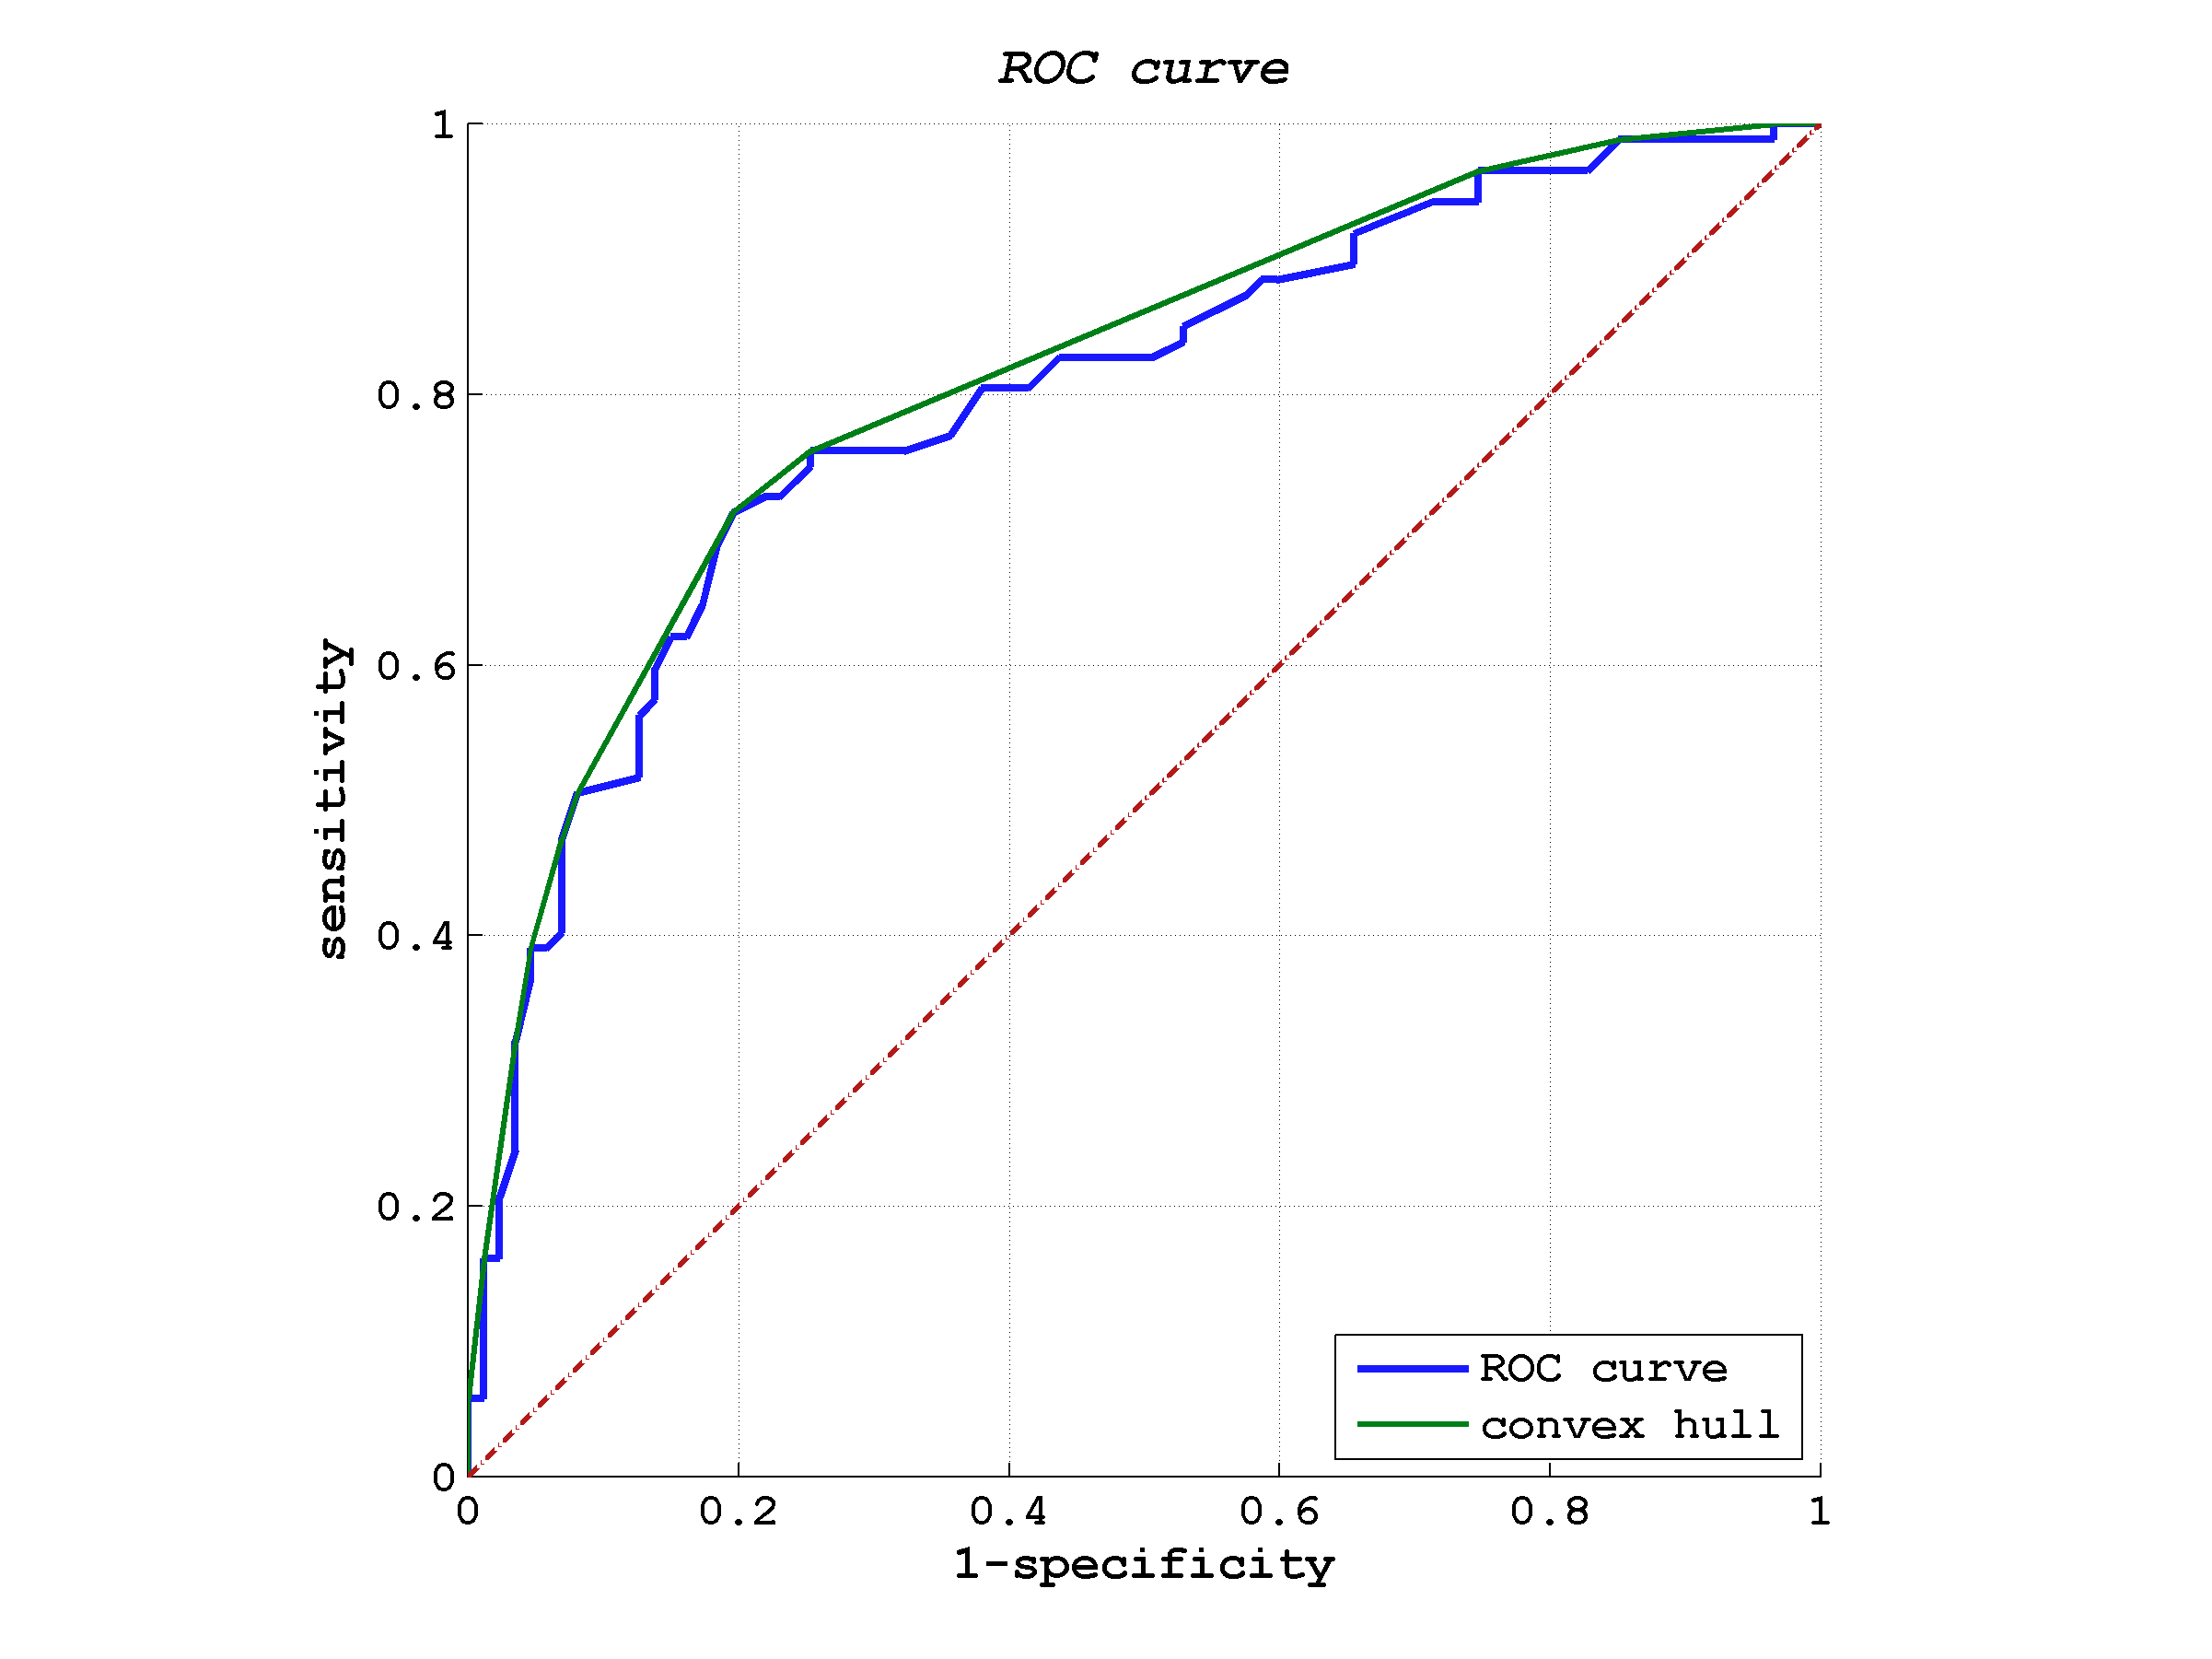
\includegraphics[width=0.84\textwidth]{./images/ROC1.png}
      \label{ch3:fig2:a}
    }\\
    %\hspace{1mm}
    \subfigure[AUC]{
      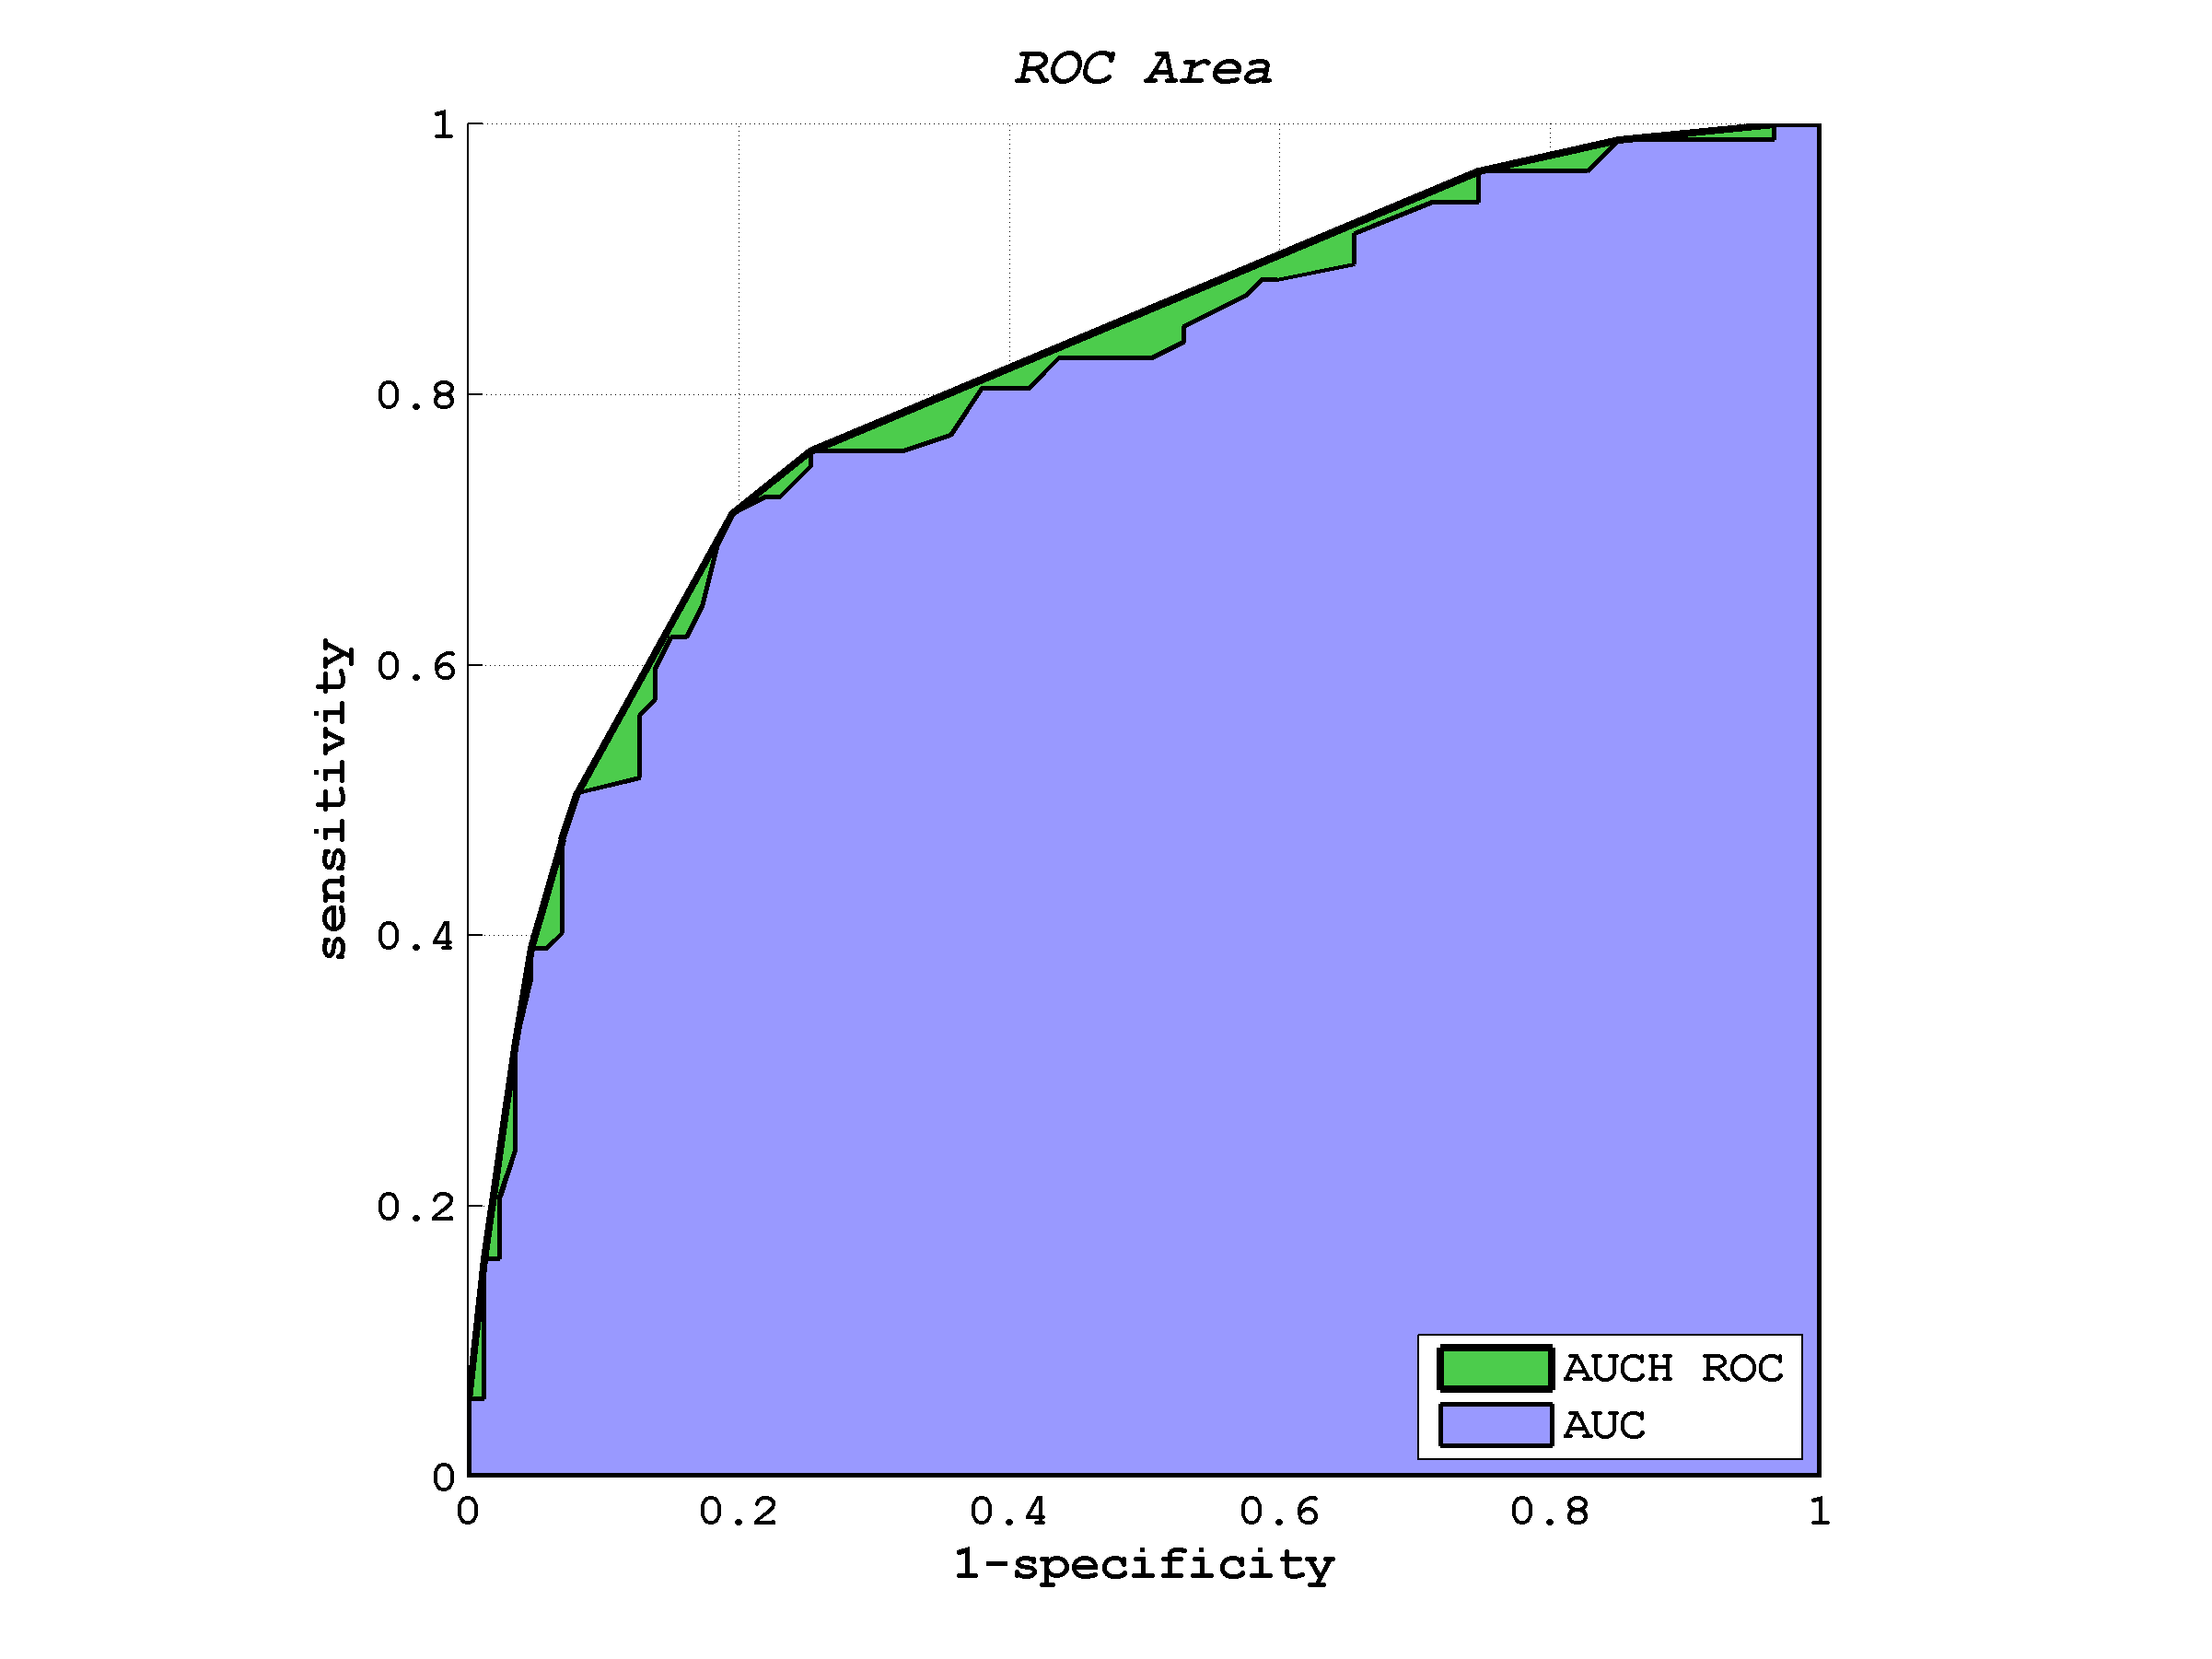
\includegraphics[width=0.84\textwidth]{./images/ROC2.png}
      \label{ch3:fig2:b}
    }
    \caption{Example of ROC curves}
    \label{ch3:fig2}
\end{figure}


The \Gls{ROC} is used to generate summary statistics. One of the often used is the area under the \Gls{ROC} curve, or \textit{AUC} (Area Under Curve)\cite{Brown200624, ROC02} (see Figure \ref{ch3:fig2:b}):
AUC is equal to the probability that a classifier will rank a randomly chosen positive instance higher than a randomly chosen negative one. The AUC can be related to other
summary statistics like the \textit{Gini coefficient} \cite{Gini} and the \textit{Mann-Withney U} \cite{MWU}.
Another common measure related to the \Gls{ROC} curve is known as the Area Under the ROC Convex Hull (\textit{AUCH ROC}, in Figure \ref{ch3:fig2:b}), which computes the area unter the convex hull of the ROC curve, as
it can be shown that any point on the line segment between two prediction results can be achieved by randomly using one or other system with probabilities proportional to the relative length of the opposite component of the segment.














% Impostazione del problema, modello
% - come si e' passati dal problema di detection al problema di classificazione
% - definizione del problema di classificazione, input, output, classi
% - come si affronta il problema di classificazione
% -- da un algoritmo (calcolo features, classificazione tramite classificatore)
% -- da un umano
% - defininzione di performance


